\documentclass[10pt]{article}

\usepackage{graphicx}
\usepackage[pdfpagelabels]{hyperref}
\usepackage{verbatim}
\usepackage[section]{placeins}
\usepackage{bookmark}
\usepackage{float}
\usepackage{tabularx}

\title{Software Release Process}
\author{Austin Green}
\date{\today\\V0.3}

\begin{document}
    \pagenumbering{Alph}
    \begin{titlepage}
    \maketitle
    \thispagestyle{empty}
    \end{titlepage}
    \pagenumbering{arabic}
	%\newpage

	%\setcounter{page}{1}
	\tableofcontents
	\newpage

    \begin{comment}
        \section{TODOs}
            \begin{itemize}
                \item revise
            \end{itemize}
        \section{Version Control}
            \begin{itemize}
                \item V0.1 - Initial Release
                \item V0.2 - Added SmarTeam kickback note
                \item V0.3 - Add Kickback Notes
            \end{itemize}
    \end{comment}

    \section{Initial Release}
        \subsection{TortoiseSVN}
            \subsubsection{Check In Code}
                Checking in code in Tortoise SVN is relatively simple. You can tell that code is modified and needs to be checked in based on the green check mark turning into a red exclamation point.
                \begin{figure}[H]
                    \centerline{
\includegraphics{References/Check.png}}
                    \figurename{ 1: Green Check Mark}
                \end{figure}
                \begin{figure}[H]
                    \centerline{
\includegraphics{References/X.png}}
                    \figurename{ 2: Red Exclamation Point}
                \end{figure}
                To check in, right click in the folder and select \emph{SVN Commit...}.
                \begin{figure}[H]
                    \centerline{
\includegraphics{References/SVN Commit.png}}
                    \figurename{ 3: SVN Commit}
                \end{figure}
                The files to be committed will be in the bottom portion of the window, selecting the check box will indicate you want to commit them. You can double click the files to bring up a diff between the current and previous versions of the file. When you are ready, type a description of the commit in the upper window and click OK.
                \begin{figure}[H]
                    \centerline{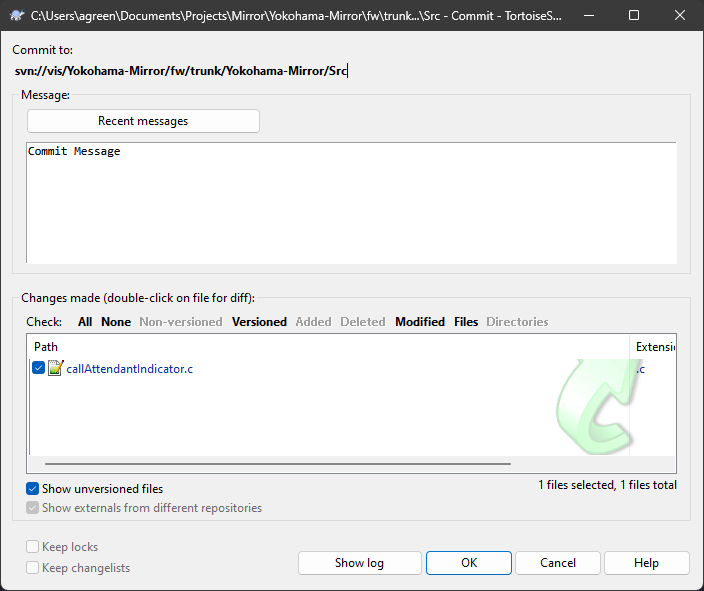
\includegraphics[width=\textwidth]{References/SVN Commit Window.png}}
                    \figurename{ 4: Commit Window}
                \end{figure}
            \subsubsection{Create Tag}
                To create a tag, go to into the trunk directory and right click and select \emph{TortoiseSVN-Branch/tag...}.
                \begin{figure}[H]
                    \centerline{
\includegraphics{References/Tag.png}}
                    \figurename{ 5: SVN Tag}
                \end{figure}
                The \emph{To path:} in the top is where to create the tag. This should be in a folder in the \emph{tags} folder with the (project)-(version)-(date) format. In the \emph{Log message} section, write a message associated with this tag. And finally, you can click \emph{Show Log} to select the version you want to include in this tag.
                \begin{figure}[H]
                    \centerline{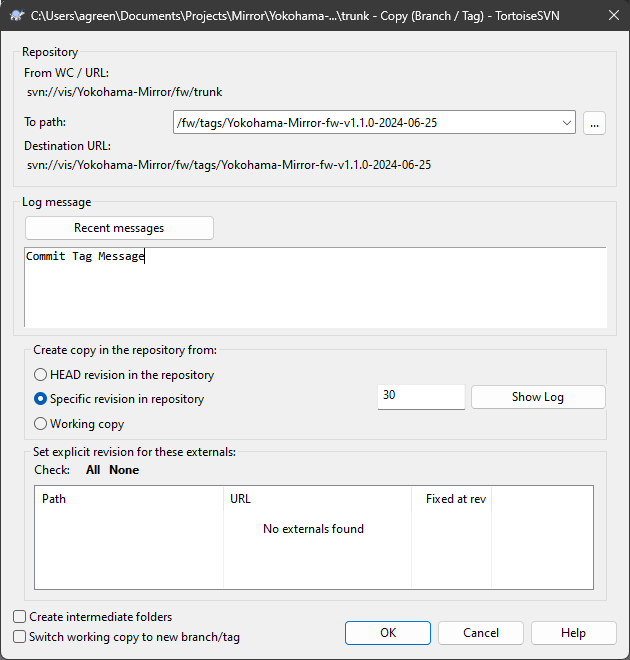
\includegraphics[width=\textwidth]{References/Tag Window.png}}
                    \figurename{ 6: Tag Window}
                \end{figure}
            \subsubsection{Release}
                To release software, create a folder in the \emph{releases} folder with the Release\_(version number) format. In this folder, create \emph{bin} and \emph{src} folders. Inside each of these folders should be a .zip file (of output files in \emph{bin} and source files in {src}), a \emph{Software Release Notes} word document, and a PDF of this document. Commit this folder to SVN using the above steps when you finish with this folder.
        \subsection{SmarTeam}
            Notoe: It is important to have all documents filled out in the way that they should be submitted before submitting an ECO, because any edits to the files will kick back the ECO to you.
            \subsubsection{Updating Files}
                SmarTeam is a bit tricky to get right so follow these steps carefully. First, in SmarTeam, navigate to your project, then the files you with to update (\emph{Design NoteBook}-\emph{Detailed Design General}-\emph{Top Level Design General}-\emph{Software}).
                \begin{figure}[H]
                    \centerline{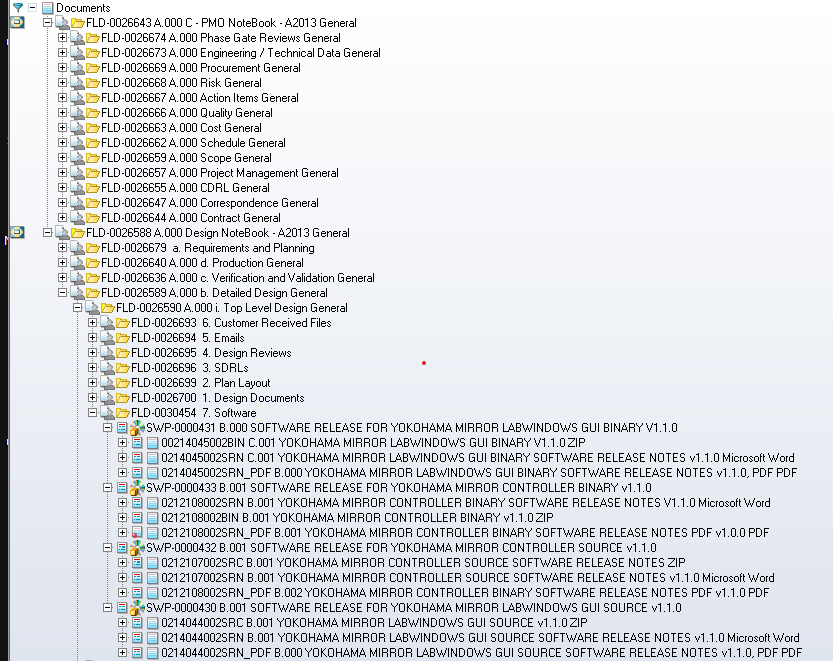
\includegraphics[width=\textwidth]{References/ST Software Folder.png}}
                    \figurename{ 7: Smart Team Software Folder}
                \end{figure}
                Next, right click on the \emph{SWP} (Software Package) and select \emph{Life Cycle}-\emph{Check Out}. if this does not exist, you will need to right click on the \emph{Software} folder and select \emph{Add}-\emph{Design}-\emph{Software Package} and fill out the information.
                \begin{figure}[H]
                    \centerline{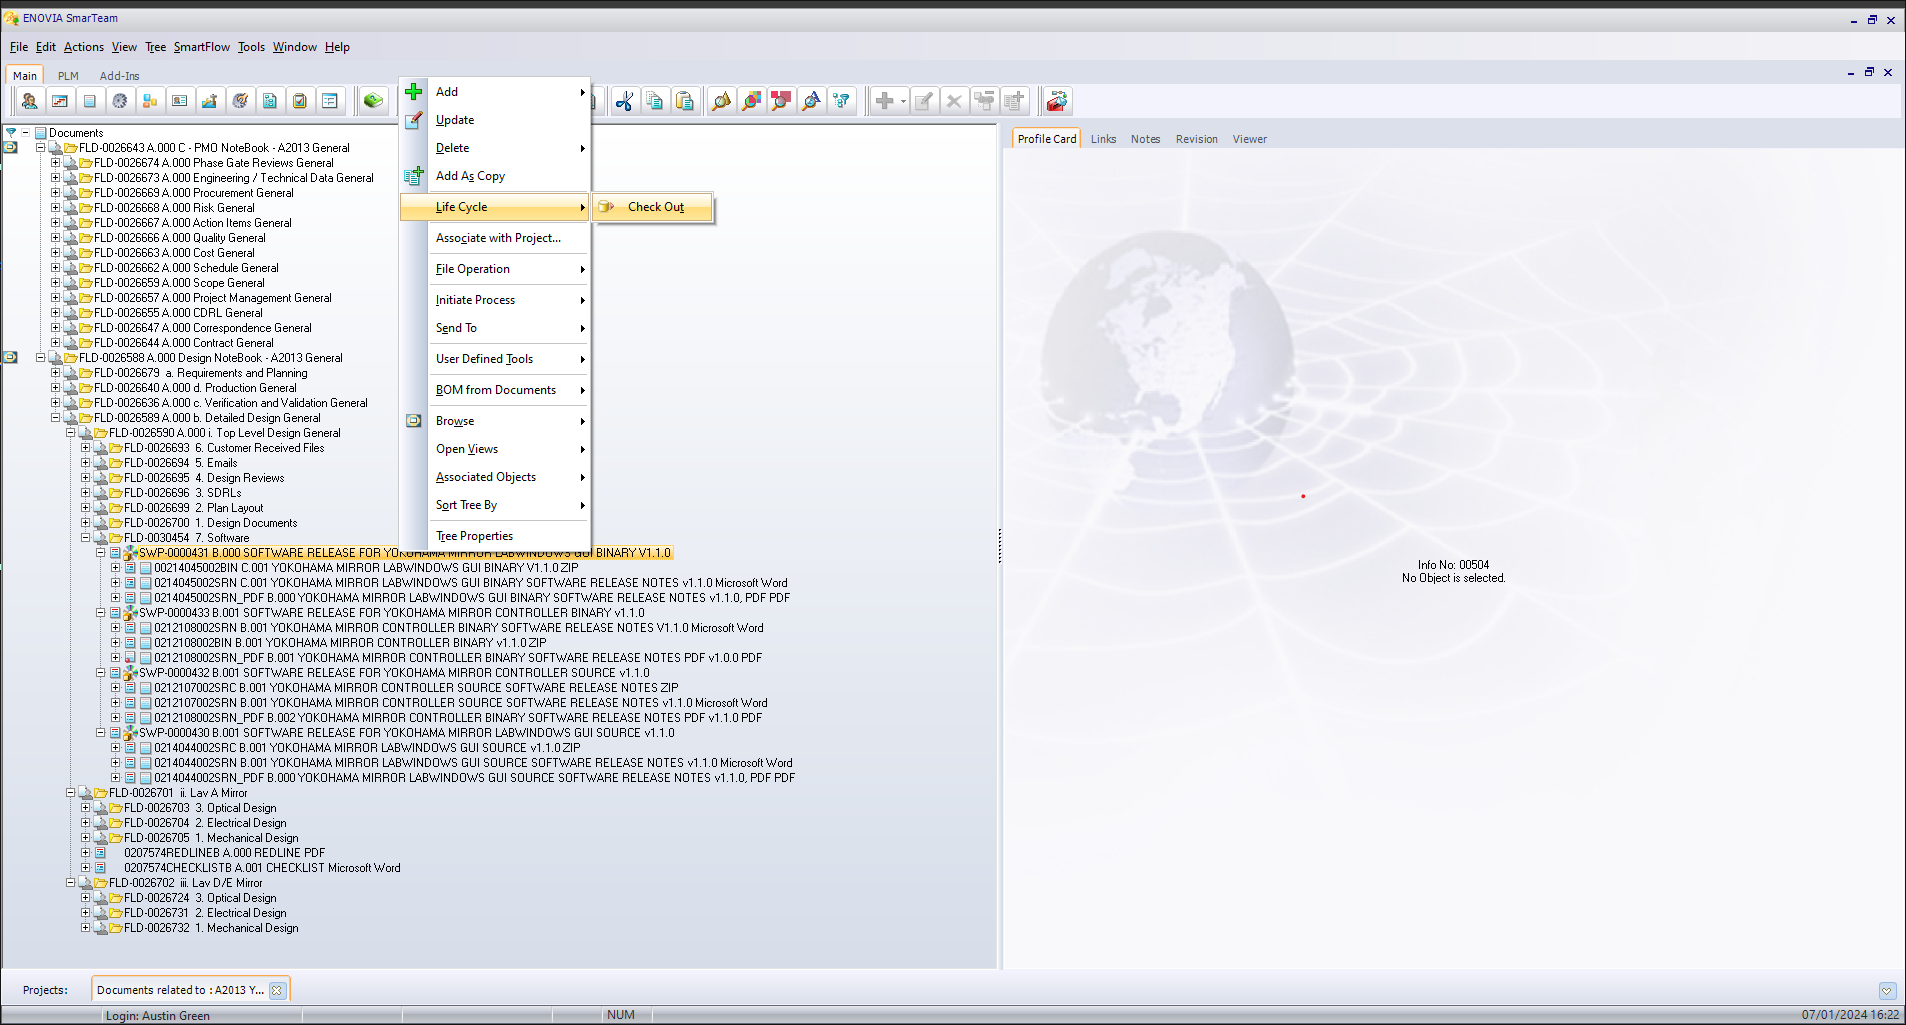
\includegraphics[width=\textwidth]{References/ST Check Out.png}}
                    \figurename{ 8: Smart Team Check Out}
                \end{figure}
                Next, right click and select \emph{Update} and update the \emph{DESCRIPTION} and \emph{COMMENTS} on the right to reflect the new version number. Additionally, update the \emph{Part Number} by increasing the number by one. Click OK when done. \\
                Next, right click and select \emph{Life Cycle}-\emph{Check Out} any files below the \emph{SWP} you are changing, paying attention to the \emph{Destination directory:} field. Click OK when you select the destination.
                \begin{figure}[H]
                    \centerline{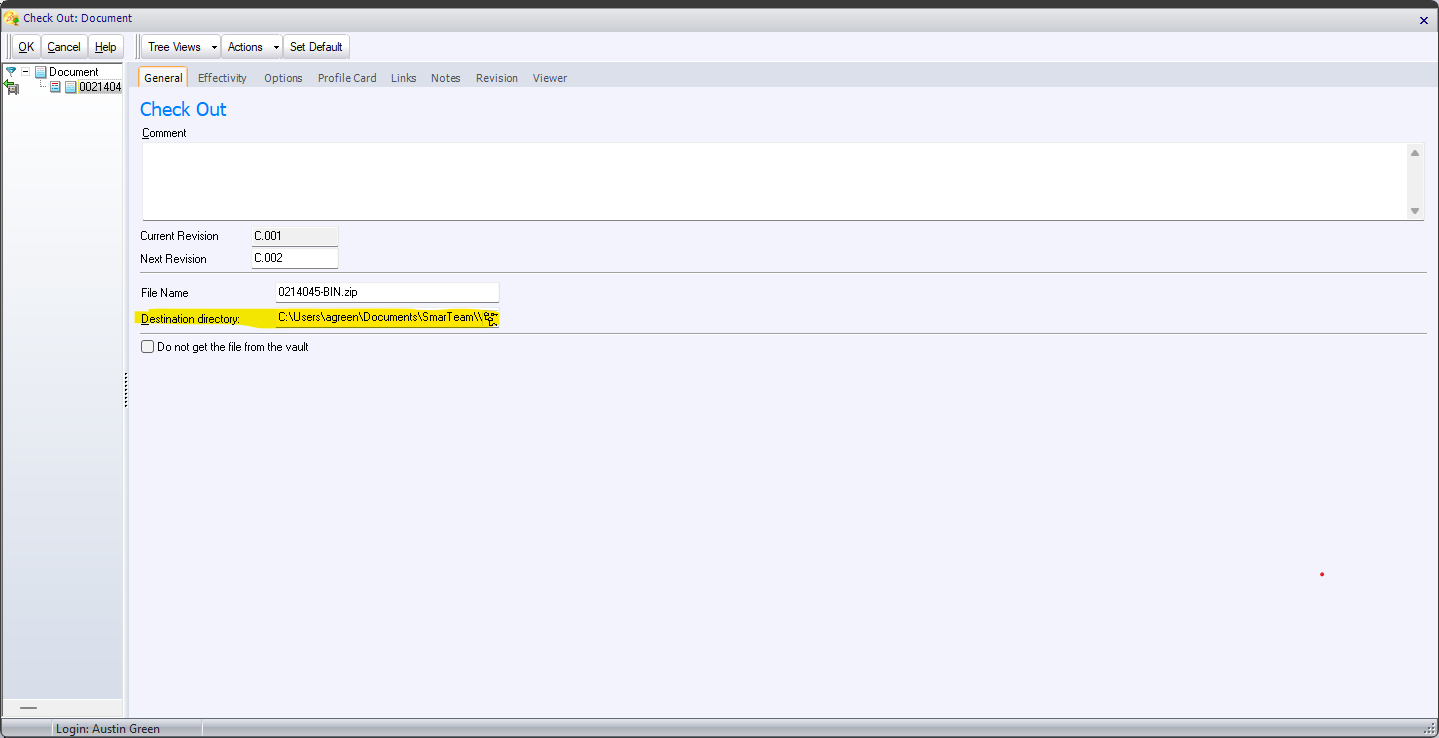
\includegraphics[width=\textwidth]{References/ST Check Out Window.png}}
                    \figurename{ 9: Check Out Window}
                \end{figure}
                If the file does not already exist in SmarTeam, right click on the \emph{SWP} and select \emph{Add}-\emph{Document} and fill out the information similar to the other documents. \\
                Next, navigate to the folder you selected as the destination folder in Windows Explorer and replace the checked out files with the ones you created in the \emph{releases} folder above. \\
                Next, back in SmarTeam, update the file similar to the way you updated the \emph{SWP} above by selecting the file and selecting \emph{Update}. You will need to update the \emph{ID} and \emph{PART NUMBER} buy increasing them by one and update the \emph{DESCRIPTION} and \emph{COMMENTS} on the right to reflect the new version number. \\
                Finally, right click and select \emph{Life Cycle}-\emph{Check In} when you are done. Add a description of the change and select \emph{OK}.
            \subsubsection{Submitting an ECO}
                There should be one ECO submitted per SWP update. When you are done updating all of the files in an SWP, right click on one of the changed files, select \emph{Initiate Process}-\emph{LAP ECO}-\emph{LAP Software - Cert/NonCert} depending.
                \begin{figure}[H]
                    \centerline{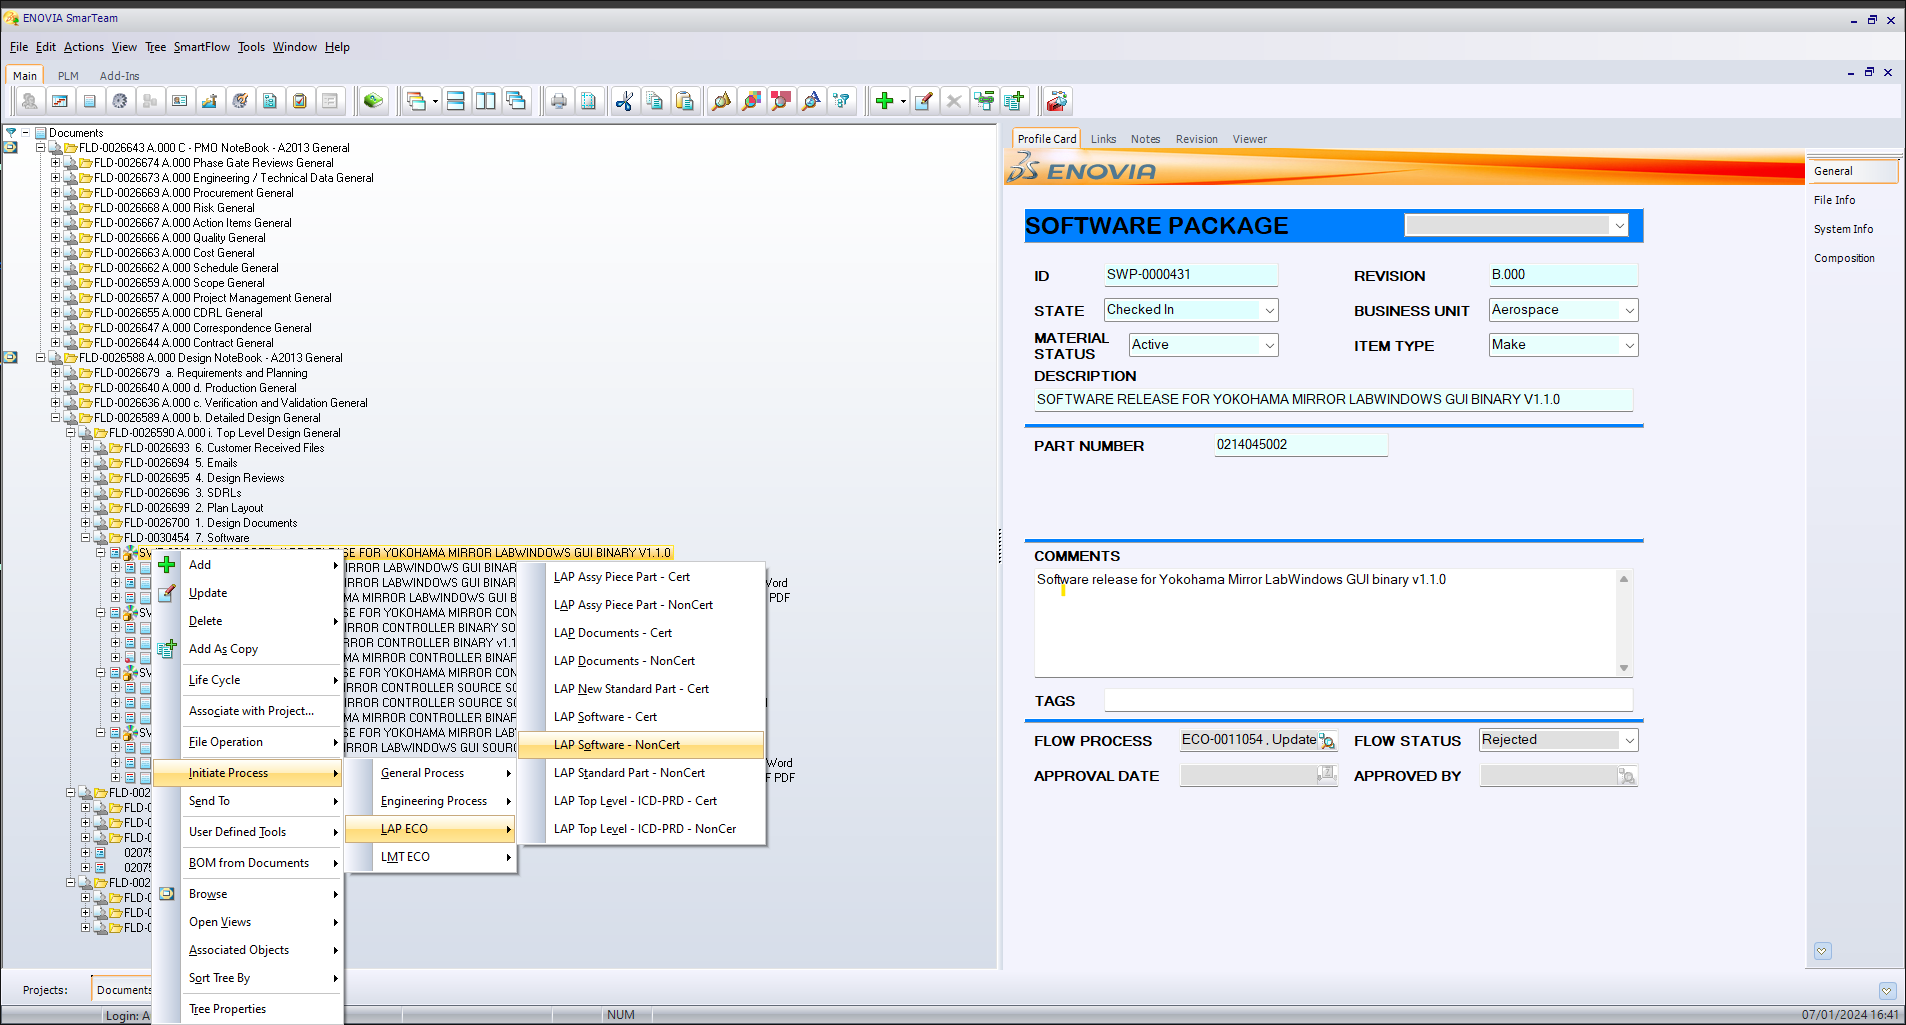
\includegraphics[width=\textwidth]{References/ST ECO Initiate Process.png}}
                    \figurename{ 10: Initiate ECO}
                \end{figure}
                This will bring up the ECO Window.
                \begin{figure}[H]
                    \centerline{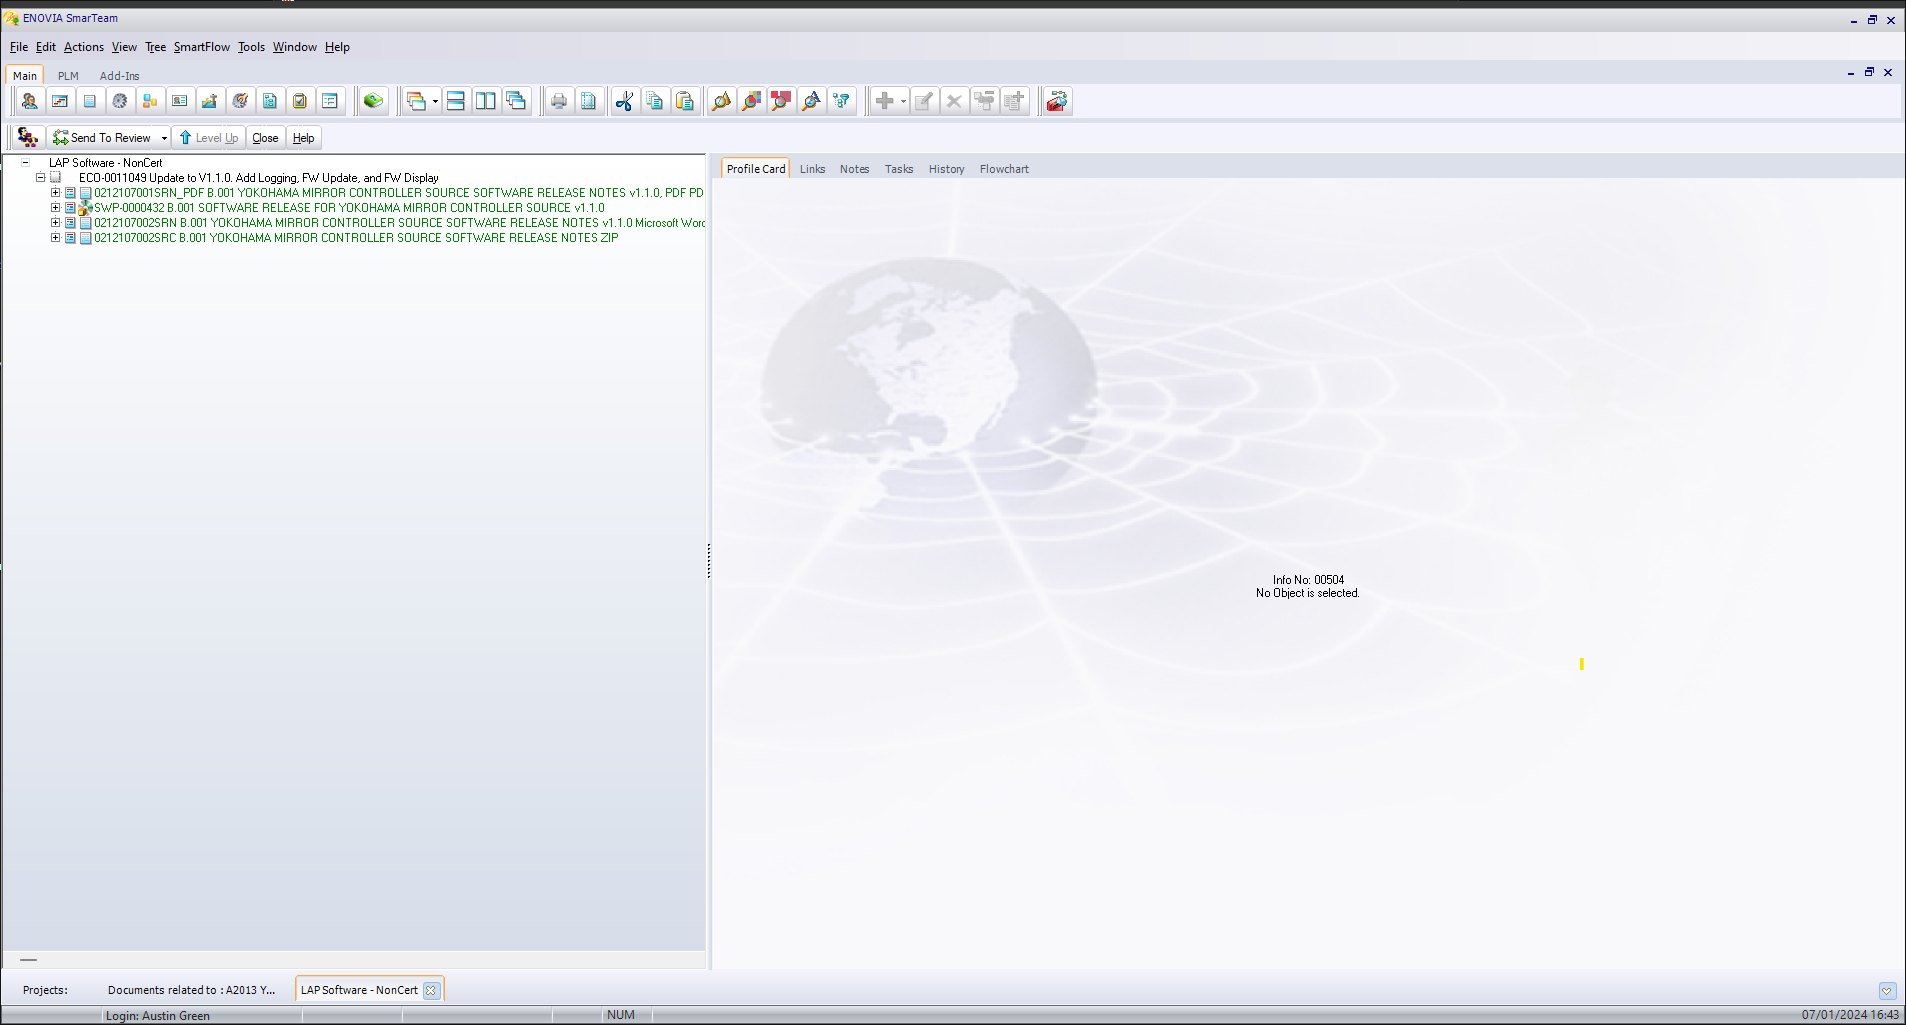
\includegraphics[width=\textwidth]{References/ST ECO Window.png}}
                    \figurename{ 11: ECO Window}
                \end{figure}
                Drag the rest of the files, including the SWP, from the Projects Documents pane (where you were checking in and out files) onto the \emph{ECO} item. \\
                Next right click the \emph{ECO} and click \emph{Update}. Fill out all the fields, the \emph{Description of Change} and \emph{Reason for Change} can be the same. The \emph{Project Number} is the number associated with the project you are in. \\
                Next, select the \emph{Flowchart} tab at the top. Right click the \emph{LAP Peer Review} box and select \emph{Executors}. From here click \emph{Add New...} and add an people that you wish to review or see the the ECO by clicking the \emph{To--} or \emph{Cc--} buttons respectively.
                \begin{figure}[H]
                    \centerline{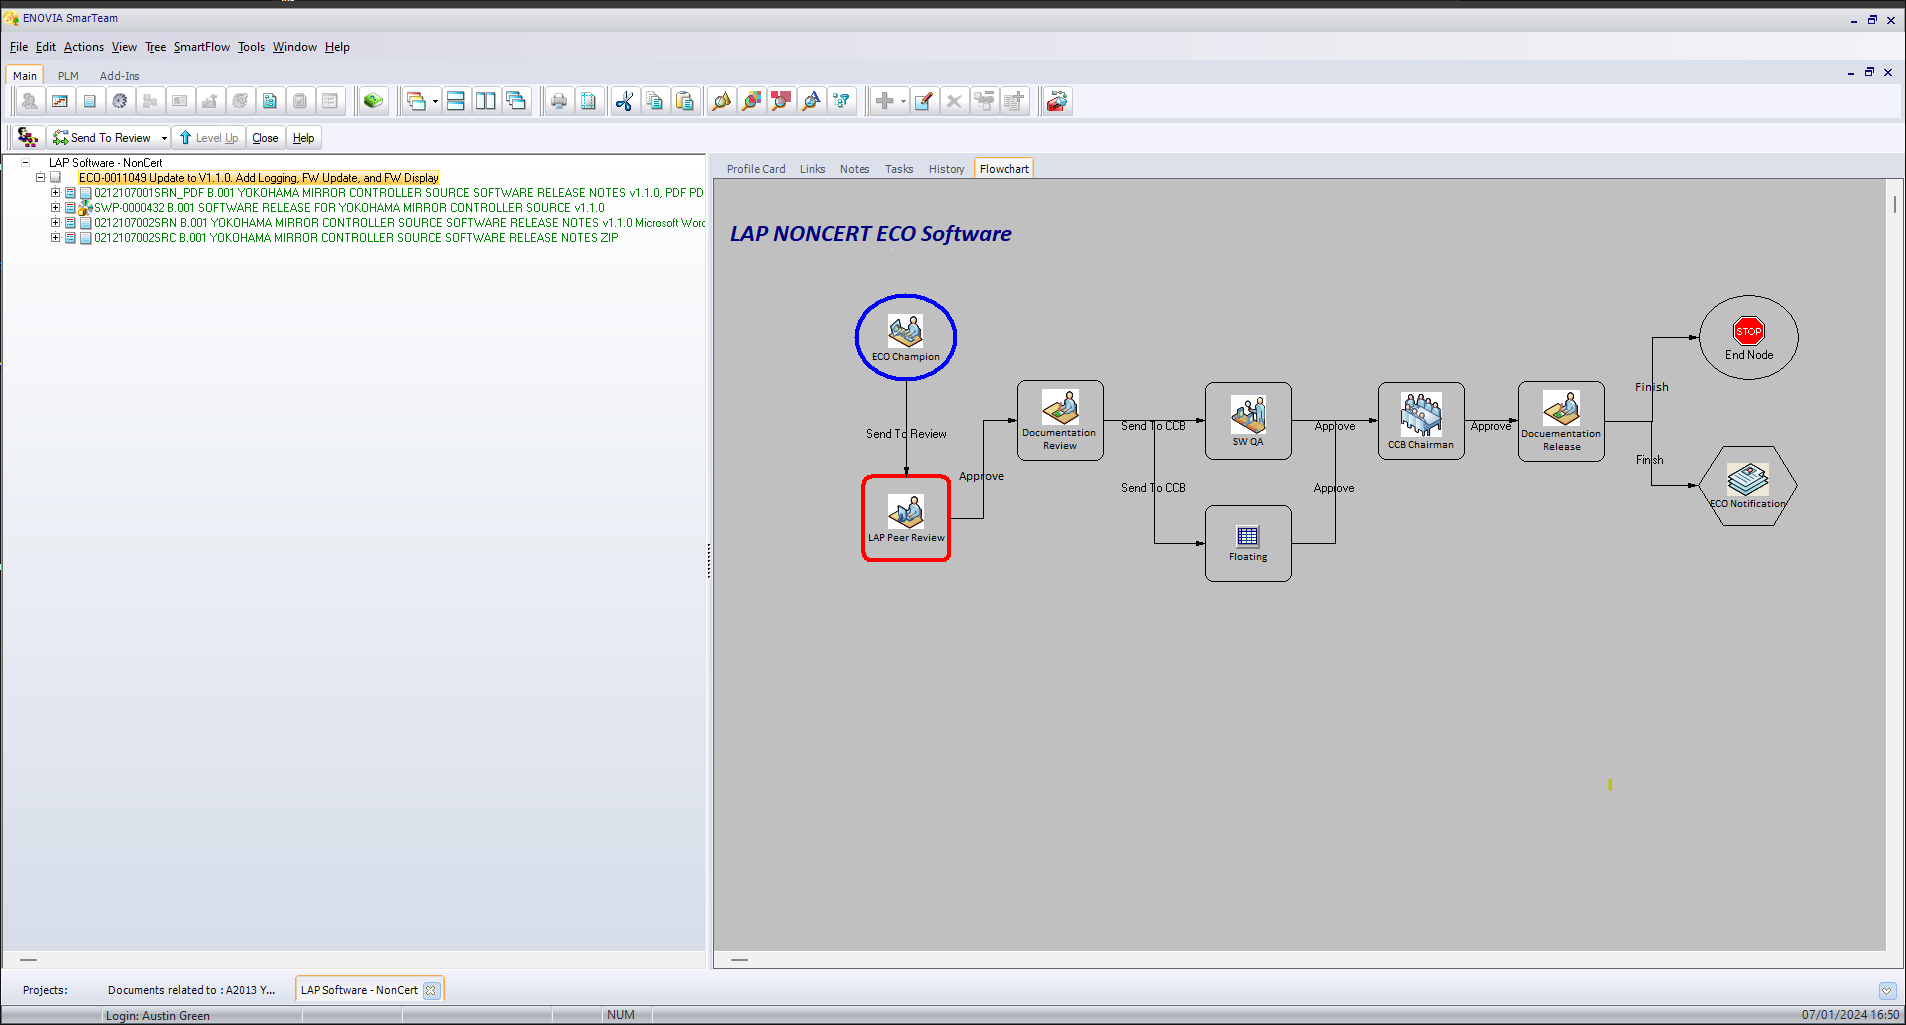
\includegraphics[width=\textwidth]{References/ST ECO Flowchart.png}}
                    \figurename{ 12: ECO Flowchart}
                \end{figure}
                \begin{figure}[H]
                    \centerline{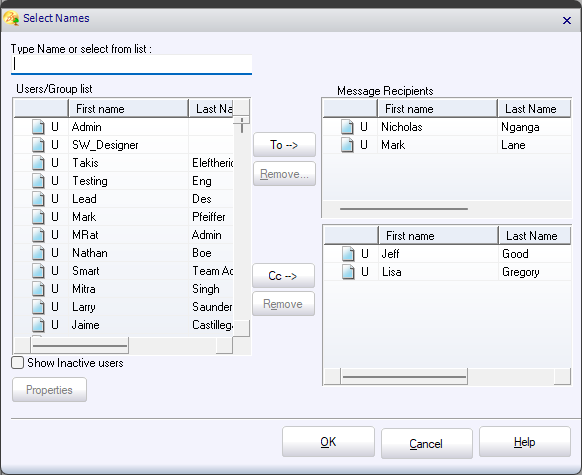
\includegraphics[width=\textwidth]{References/ST ECO Select Names.png}}
                    \figurename{ 13: Select Names}
                \end{figure}
                When you are finished, select the \emph{Send To Review} button in the top left and click \emph{OK}. This will pull up an Outlook email which you can go ahead and send. You have now submitted an ECO!
    \section{ECO Kickback}
        If an ECO is kicked back to you (rejected) it will show up in your SmarTeam inbox.
        \begin{figure}[H]
            \centerline{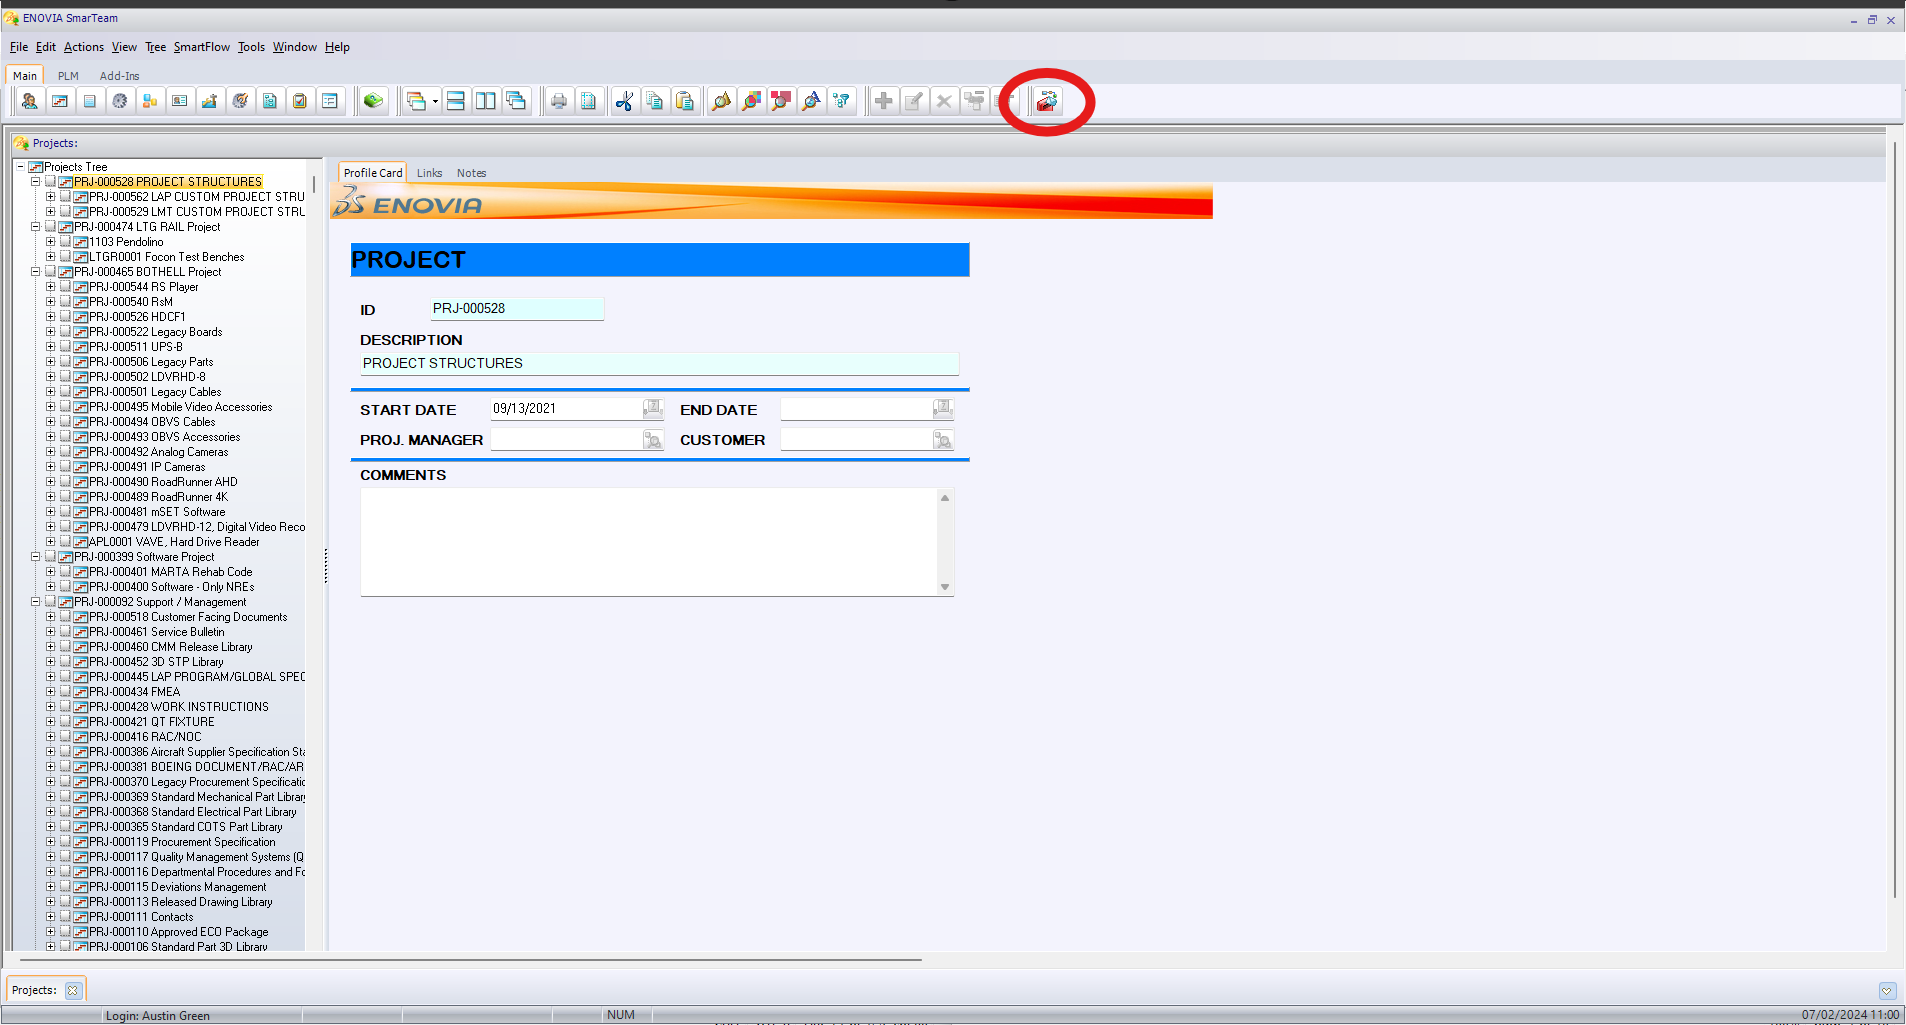
\includegraphics[width=\textwidth]{References/ST Inbox.png}}
            \figurename{ 14: SmarTeam Inbox}
        \end{figure}
        If you double click on the message, it will open up the ECO. Resubmitting the ECO is easy, all the files you submitted are already in there, so if you need to change any go through the same Checkout-Checkin process listed above. Likewise, if you need to add more files, go through the Add files process listed above. Any changes made to the files should automatically be reflected in the ECO. All you need to do from here is double check that the documents in the ECO are correct, and if not replace them. From there click the \emph{Send To Review} button again.
\end{document}